
% \ifenglish
% 
% Legal Notes:
% 
% There is no warranty for any part of the documented software. The authors have taken care in the
% preparation of this thesis, but make no expressed or implied warranty of any kind and assume no
% responsibility for errors or omissions. No liability is assumed for incidental or consequential
% damages in connection with or arising out of the use of the information or programs contained here.
% 
% \else
% 
% Notas legais:
% 
% Não há garantia para qualquer parte do software documentado. Os autores tomaram cuidado na
% preparação desta tese, mas não fazem nenhuma garantia expressa ou implícita de qualquer tipo e não
% assumem qualquer responsabilidade por erros ou omissões. Não se assume qualquer responsabilidade por
% danos incidentais ou consequentes em conexão ou decorrentes do uso das informações ou programas aqui
% contidos.
% 
% \fi


% http://portalbu.ufsc.br/ficha
% http://portal.bu.ufsc.br/servicos/ficha-de-identificacao-da-obra/
\begin{fichacatalografica}
    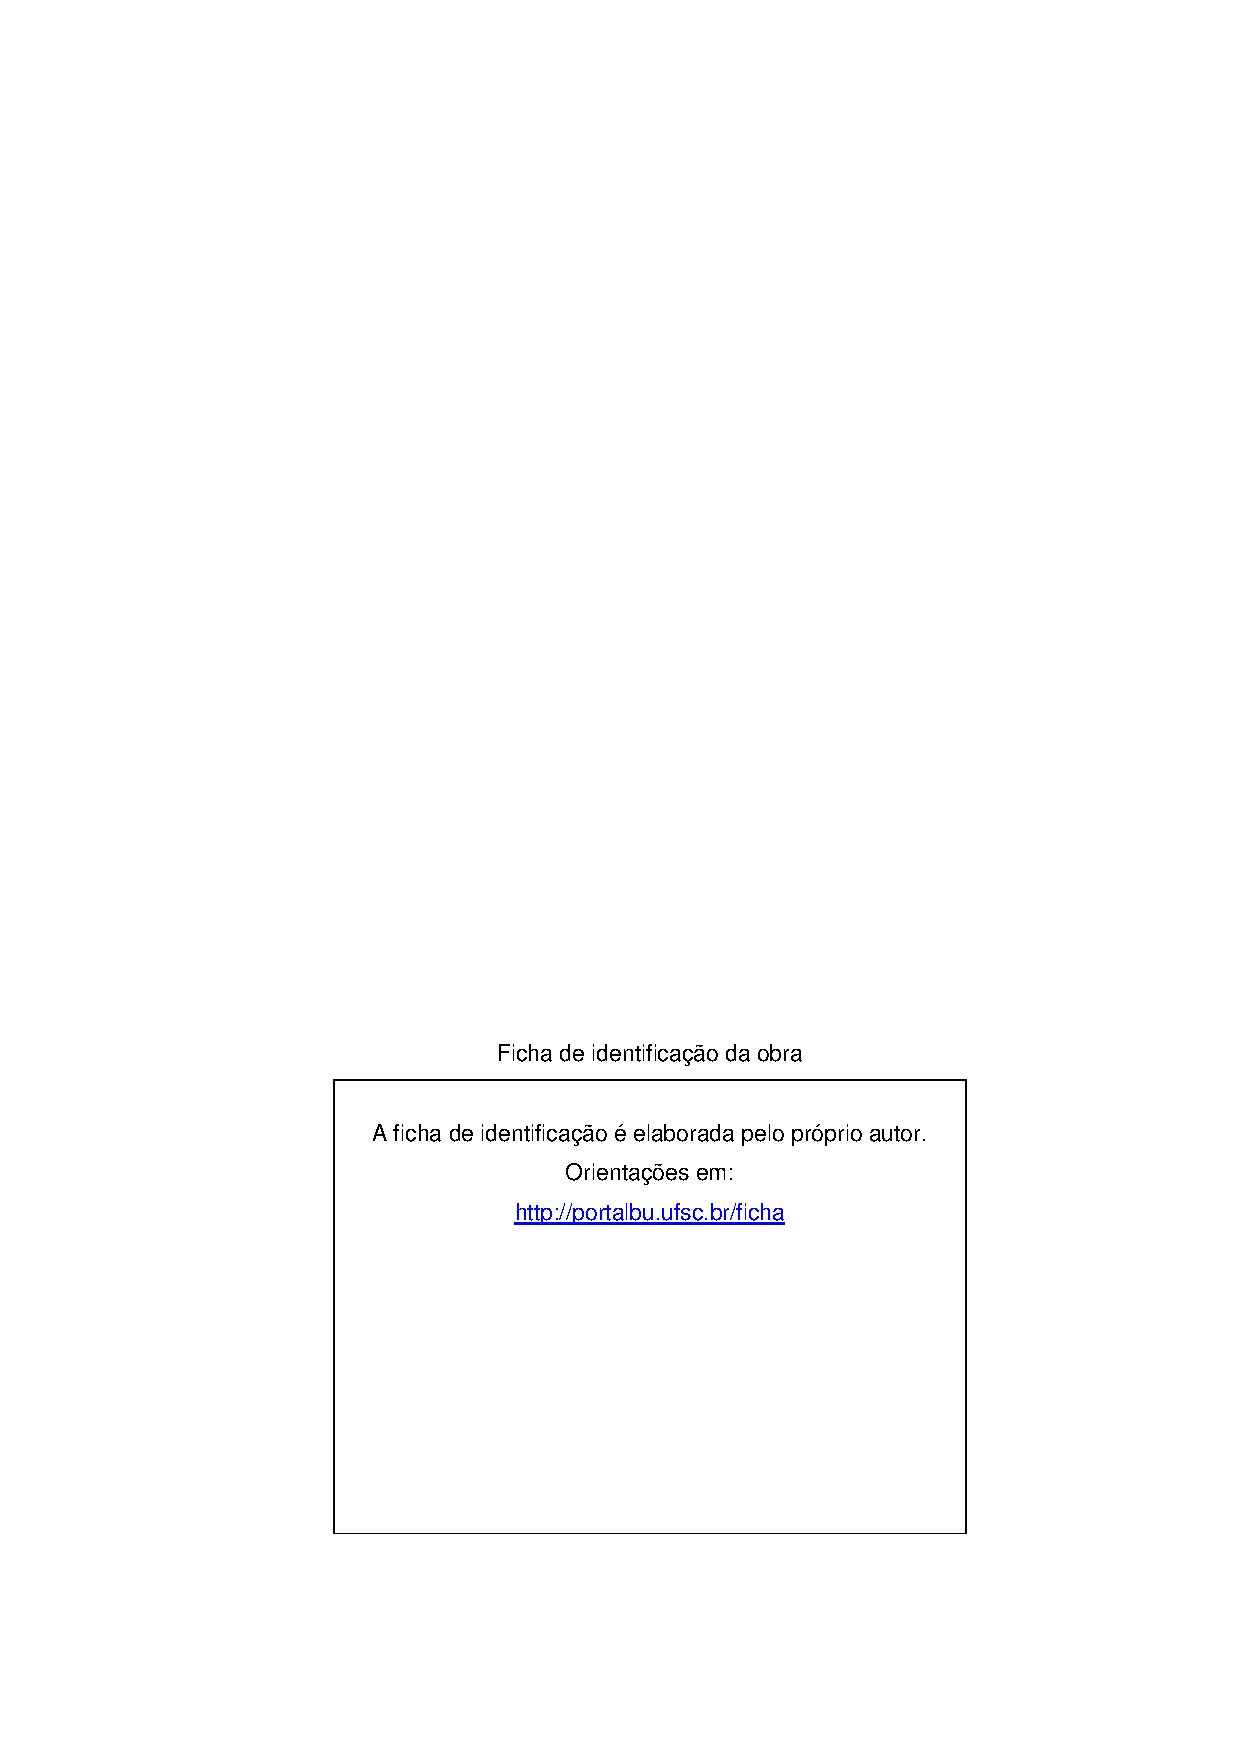
\includepdf{pictures/Ficha_Catalografica.pdf}

    % \vspace*{\fill}

    % \begin{center}

    %     \lang
    %     {Cataloging at source by the University Library of the Federal University of Santa Catarina.}
    %     {Catalogação na fonte pela Biblioteca Universitária da Universidade Federal de Santa Catarina.}

    %     \lang
    %     {File compiled at \currenttime h of the day \today.}
    %     {Arquivo compilado às \currenttime h do dia \today.}

    %     \framebox[\textwidth]
    %     {
    %         % https://tex.stackexchange.com/questions/369918/use-the-value-of-title-with-removed-linebreak
    %         \begin{minipage}{0.98\textwidth}
    %         \begingroup \let\\=\space

    %             \ttfamily
    %             \imprimirautor

    %             \hspace{0.5cm} \imprimirtitulo%
    %             \ifnotempty{\imprimirsubtitulo}{~:~\imprimirsubtitulo}%
    %             ~/~\imprimirautor%
    %             ;~\imprimirorientadorRotulo,~\imprimirorientador%
    %             \ifnotempty{\imprimircoorientador}{;~\imprimircoorientadorRotulo,~\imprimircoorientador}%
    %             ~--~\imprimirlocal,~\imprimirdata.

    %             % Prints how much pages there are on the document and links to the last page
    %             \hspace{0.5cm} \pageref{LastPage} p.
    %             \bigskip

    %             \hspace{0.5cm} \imprimirtipotrabalho~--~\imprimirinstituicao,
    %             \imprimircentro,~\imprimirprograma.
    %             \bigskip

    %             \hspace{0.5cm} \lang{Includes references}{Inclui referências}
    %             \bigskip

    %             % https://tex.stackexchange.com/questions/54055/using-lower-case-roman-numerals-in-enumerate-lists
    %             % https://tex.stackexchange.com/questions/61811/how-to-define-inparaenum-in-the-preamble
    %             \hspace{0.5cm}
    %             \begin{inparaenum}
    %                 \lang{\palavraschaveinglescomvirgula}{\palavraschaveportuguescomvirgula}%
    %             \end{inparaenum}%
    %             \begin{inparaenum}[I.]
    %                 \item \imprimirorientador~
    %                 \ifnotempty{\imprimircoorientador}{\item \imprimircoorientador~}
    %                 \item \imprimirprograma~
    %                 \item \imprimirtitulo~
    %             \end{inparaenum}%
    %             \bigskip

    %             \hspace{7.75cm} CDU 02:141:005.7

    %         \endgroup
    %         \end{minipage}
    %     }

    % \end{center}

\end{fichacatalografica}

